\documentclass[tikz,border=4pt]{standalone}
\usepackage{amsmath,amssymb}
\usetikzlibrary{arrows.meta,decorations.markings}

\begin{document}
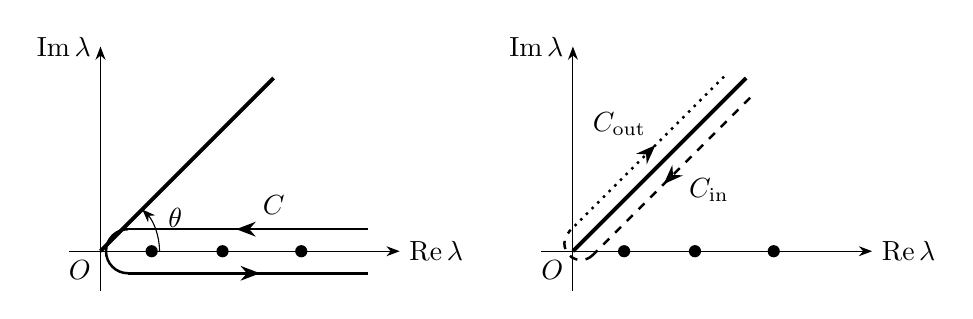
\begin{tikzpicture}[
  >=Stealth,
  font=\normalsize,
  axis/.style={line width=0.4pt},
  curve/.style={line width=0.9pt},
  branch/.style={line width=1.4pt},
  midarrow/.style={postaction={decorate,decoration={markings,mark=at position 0.55 with {\arrow{Stealth}}}}}
]
  % Left panel: Contour C
  \begin{scope}
    \draw[axis,->] (-0.4,0) -- (3.8,0) node[right] {$\operatorname{Re}\lambda$};
    \draw[axis,->] (0,-0.5) -- (0,2.6) node[left] {$\operatorname{Im}\lambda$};
    \node[below left] at (0,0) {$O$};

    % Branch cut at angle theta = 45 deg
    \draw[branch] (0,0) -- (2.2,2.2);
    \draw[axis,->] (0.75,0) arc (0:45:0.75);
    \node at (0.95,0.42) {$\theta$};

    % Eigenvalues on positive real axis
    \foreach \x in {0.65, 1.55, 2.55} {
      \fill (\x,0) circle (2.2pt);
    }

    % Contour C enclosing positive real axis (clockwise or counterclockwise? Let's match original:
    % Wait: in original figure, top goes LEFT (from +inf to 0) and bottom goes RIGHT (from 0 to +inf) -> counterclockwise around eigenvalues!
    \draw[curve,midarrow] (3.4,0.28) -- (0.35,0.28);
    \draw[curve] (0.35,0.28) arc (90:270:0.28);
    \draw[curve,midarrow] (0.35,-0.28) -- (3.4,-0.28);
    \node[above] at (2.2,0.34) {$C$};
  \end{scope}

  % Right panel: Deformed contours C_in and C_out along branch cut
  \begin{scope}[xshift=6.0cm]
    \draw[axis,->] (-0.4,0) -- (3.8,0) node[right] {$\operatorname{Re}\lambda$};
    \draw[axis,->] (0,-0.5) -- (0,2.6) node[left] {$\operatorname{Im}\lambda$};
    \node[below left] at (0,0) {$O$};

    % Branch cut at angle 45 deg
    \draw[branch] (0,0) -- (2.2,2.2);

    % Eigenvalues on positive real axis
    \foreach \x in {0.65, 1.55, 2.55} {
      \fill (\x,0) circle (2.2pt);
    }

    % C_in (dashed, below branch cut, going toward origin)
    \draw[curve,dashed,midarrow] (2.25,1.95) -- (0.25,-0.05);
    \node[below right] at (1.35,1.05) {$C_{\mathrm{in}}$};

    % Small arc around origin
    \draw[curve,dashed] (0.25,-0.05) arc (-45:-225:0.21);

    % C_out (dotted, above branch cut, going away from origin)
    \draw[curve,dotted,midarrow] (-0.05,0.25) -- (1.95,2.25);
    \node[above left] at (1.05,1.35) {$C_{\mathrm{out}}$};
  \end{scope}
\end{tikzpicture}
\end{document}
